% IEEE-style conference layout (two columns, 10pt Times). IEEEtran.cls was not available
% offline, so the layout is reproduced with standard packages; the source compiles with pdflatex.
\documentclass[10pt,twocolumn,letterpaper]{article}
\usepackage[top=0.75in,bottom=1in,left=0.625in,right=0.625in,columnsep=0.25in]{geometry}
\usepackage[T1]{fontenc}
\usepackage{mathptmx}
\usepackage{graphicx,booktabs,amsmath,url}
\usepackage[hidelinks]{hyperref}
\usepackage[font=footnotesize,labelsep=period]{caption}
\usepackage{titlesec}
\usepackage{balance}
\renewcommand{\thesection}{\Roman{section}}
\renewcommand{\thesubsection}{\Alph{subsection}}
\titleformat{\section}{\normalfont\scshape\centering}{\thesection.}{0.5em}{}
\titleformat{\subsection}{\normalfont\itshape}{\thesubsection.}{0.5em}{}
\titlespacing*{\section}{0pt}{8pt}{4pt}
\titlespacing*{\subsection}{0pt}{6pt}{3pt}
\renewcommand{\tablename}{TABLE}
\renewcommand{\thetable}{\Roman{table}}
\renewcommand{\figurename}{Fig.}
\setlength{\parskip}{0pt}
\pagestyle{plain}

\begin{document}
\twocolumn[
\begin{center}
{\LARGE Did the ABPS Rollout Alter MGNREGA Worker Deletions?\par}
\vspace{2pt}
{\large A Within-State Difference-in-Differences Study with Validation of the Exposure Proxy\par}
\vspace{10pt}
{\normalsize Vivaan Atharva (PES1UG24AM071) \quad Vivek Varma (PES1UG24AM070)\par}
\vspace{2pt}
{\small\itshape Team ByteMe, Advanced Data Analytics (UE24AM343AB1), Dept. of CSE (AI \& ML), PES University, Bengaluru, India\par}
\vspace{12pt}
\end{center}
]

\noindent\textbf{\textit{Abstract}---In January 2023 India's rural employment guarantee scheme (MGNREGA) moved all wage payments to the Aadhaar-Based Payment System (ABPS), and recorded worker deletions rose from 15.0 million in FY2021--22 to 51.9 million in FY2022--23. We ask whether districts with more pre-policy account-conversion friction, proxied by the FY2020--21 share of post-office or joint accounts, saw larger rises in deletions. Using 15 district-level tables extracted from the scheme's Management Information System (MIS) for about 710 districts, we first validate the proxy in a pre-registered Stage~0: within states, one standard deviation more exposure predicts a 0.12--0.15 SD lower pre-mandate ABPS share of wages (effective $F$ = 29--65 in three of four years, stable when any state is dropped), but the relationship is weak (within-state $R^2 \approx 3\%$) and concentrated in high-exposure districts. Stage~1 estimates a difference-in-differences model with district and state$\times$year fixed effects. High-friction districts (top within-state decile) show no larger rise in deletions in FY2022--23: $-1.2$ per 1,000 workers (SE 9.3, 95\% CI $[-19.4, 17.0]$), against an average jump from 34 to 120 per 1,000. Twelve of fourteen specifications are not significant. Because the ABPS order came late in FY2022--23 and became binding only in FY2023--24, the main extension is to add later years.}

\vspace{4pt}
\noindent\textbf{\textit{Index Terms}---difference-in-differences, proxy validation, fixed effects, Poisson pseudo-maximum likelihood, MGNREGA, Aadhaar, public data.}

\section{Introduction}
The Mahatma Gandhi National Rural Employment Guarantee Act (MGNREGA) offers up to 100 days of wage work a year to rural households. On 30 January 2023 the Ministry of Rural Development (MoRD) ordered that wages be paid only through ABPS, which routes money to the bank account linked to a worker's Aadhaar number. After five extensions, the requirement became binding on 1 January 2024. ABPS needs three links per worker: Aadhaar seeded to the job card, Aadhaar seeded to the bank account (with eKYC), and the account's bank recorded in the National Payments Corporation of India (NPCI) mapper.

Official replies to Parliament report that all-worker deletions rose from 15.0 million in FY2021--22 to 51.9 million in FY2022--23, and that 8.62 million and 6.89 million \emph{active} workers were deleted in FY2022--23 and FY2023--24. MoRD guidance states that a job card should not be deleted only because a worker is not ABPS-eligible. Deletions are administrative records, so a rise is not by itself evidence of wrongful exclusion; the question is whether deletions rose \emph{more} where conversion to ABPS was harder.

We measure conversion difficulty with the FY2020--21 share of a district's worker accounts that are post-office or joint accounts. A post-office account sits on a separate payment rail and may need re-seeding before an NPCI mapping exists; a joint account can carry the NPCI mapping of at most one holder. Reviewers of our project proposal pointed out that the causal claim rests on this proxy, so we validate it empirically before using it (Stage~0), with pass rules fixed in advance, and only then estimate the difference-in-differences (Stage~1).

\section{Related Work}
Biometric payment reforms in India have been studied mainly for payment performance; Muralidharan, Niehaus and Sukhtankar~\cite{mns2016} show that smartcard-based payments in Andhra Pradesh reduced leakage and delays. Public work specific to ABPS and MGNREGA deletions is largely descriptive. Methodologically, we follow the difference-in-differences literature: continuous or dose treatments need stronger parallel-trends conditions~\cite{cgs2024}; when the observed treatment is only a proxy, the reduced-form effect can be rescaled by a first stage (fuzzy DiD,~\cite{dcdh2018}); inference should be clustered at the level of shared shocks~\cite{bdm2004}; and pre-trends can be bounded rather than merely tested~\cite{rr2023}. Count outcomes are modelled with Poisson pseudo-maximum likelihood (PPML) with high-dimensional fixed effects~\cite{cgz2020}.

\section{Data}
All data come from the MGNREGA MIS (NREGASoft) national report index, selected for all states and drilled down to district level for each financial year, pulled on 29 October 2026. Raw pages are archived verbatim with fetch times. We use five reports (Table~\ref{tab:data}). We checked empirically whether each report is year-specific by pulling it for two financial years: two eligibility reports return identical totals for every year, so they describe \emph{today's} database, measured after the deletion wave.

\begin{table}[t]
\centering\footnotesize
\caption{MIS reports used (district level)}\label{tab:data}
\begin{tabular}{@{}p{2.9cm}p{1.9cm}p{2.9cm}@{}}
\toprule
Report & Behaviour & Role\\
\midrule
Accounts by bank / post office, individual / joint & Year-specific & Exposure, FY2020--21; wage denominator\\
Deleted job cards / applicants & Cumulative stock & Outcome (year-on-year change)\\
Aadhaar-based payment report & Year-specific & Pre-mandate readiness, FY2018--19 to 2021--22\\
Aadhaar status with NPCI mapper & Today only & Current readiness\\
Aadhaar authentication status & Today only & Current eligible count\\
\bottomrule
\end{tabular}
\end{table}

\textbf{Outcome.} Annual worker deletions are the change in the cumulative count of workers tagged as deleted; the rate is per 1,000 non-deleted registered workers at the start of the year. Rows with negative net deletions (restorations or record revisions; 207 district-years) are excluded and counted, and rates are winsorised at the 1st and 99th percentiles. \textbf{Exposure.} $E_d$ = (post-office + joint bank accounts) / all worker accounts in FY2020--21. Its median is 1.2\%, its 90th percentile 14.5\%, and 61\% of its variance lies within states. \textbf{Readiness.} The ABPS share of wages is the ABPS processed amount divided by total wages paid to accounts in the same year.

\textbf{Quality checks.} In every table and state, the district rows sum exactly to the state's printed total (0 mismatches). National deletions rebuilt from the MIS stocks reach 97\% of the official two-year total for FY2021--22 and FY2022--23, and state totals rank-correlate at 0.92 with the active-worker series in Lok Sabha USQ~294 (Fig.~\ref{fig:audit}). The MIS records 5.7 million fewer deletions than the official figure in FY2021--22 and 3.9 million more in FY2022--23, which we treat as a timing shift. True zeros stay zeros, blanks stay missing, and no outcome is imputed. The final panel has 2,594 district-years in 706 districts and 33 states and union territories, FY2019--20 to FY2022--23.

\begin{figure}[t]
\centering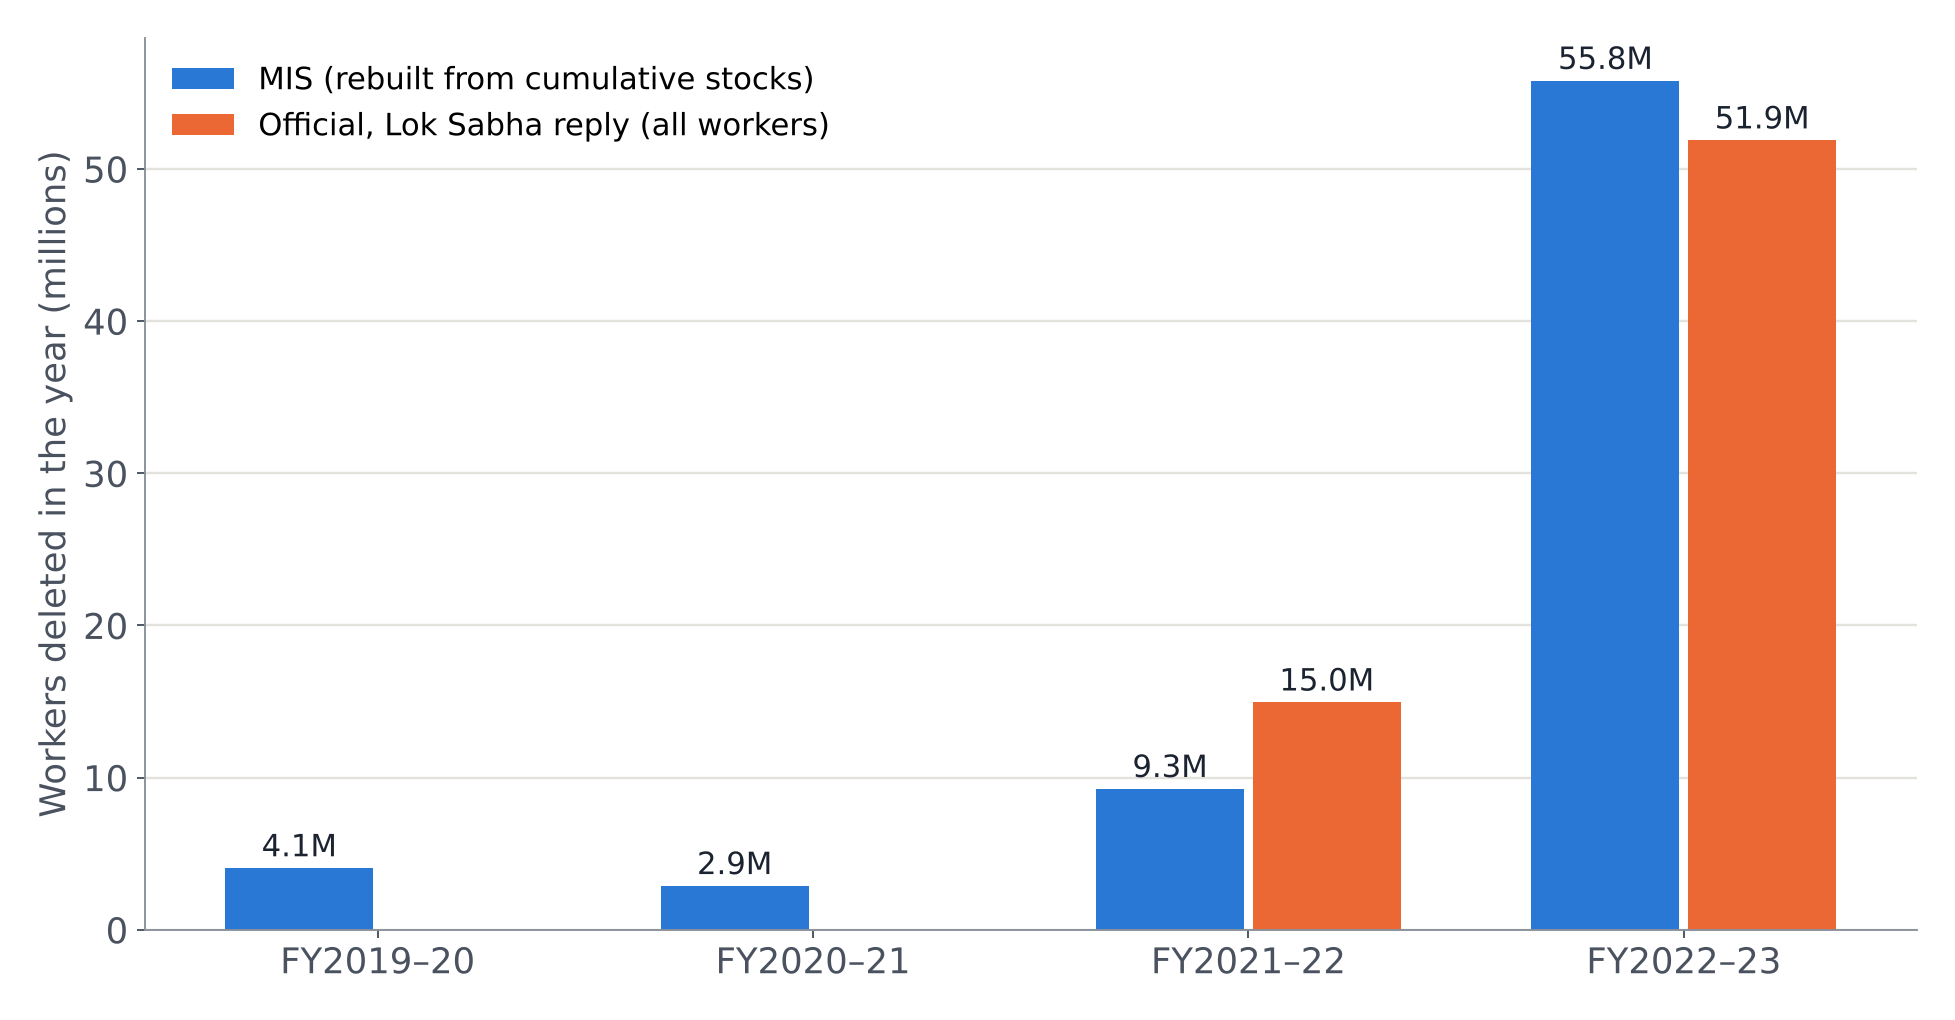
\includegraphics[width=\columnwidth]{fig_deletions_audit.png}
\caption{Workers deleted per year: rebuilt from MIS cumulative stocks vs official all-worker figures.}\label{fig:audit}
\end{figure}

\section{Methodology}
Fig.~\ref{fig:design} summarises the pipeline. All estimators (fixed-effects OLS by alternating projections, PPML by iteratively reweighted least squares, CR1 cluster-robust standard errors) were written for this project and checked on simulated panels with known effects: the estimates recover the true coefficients, and a 5\% test rejects a true null 3\% of the time.

\begin{figure*}[t]
\centering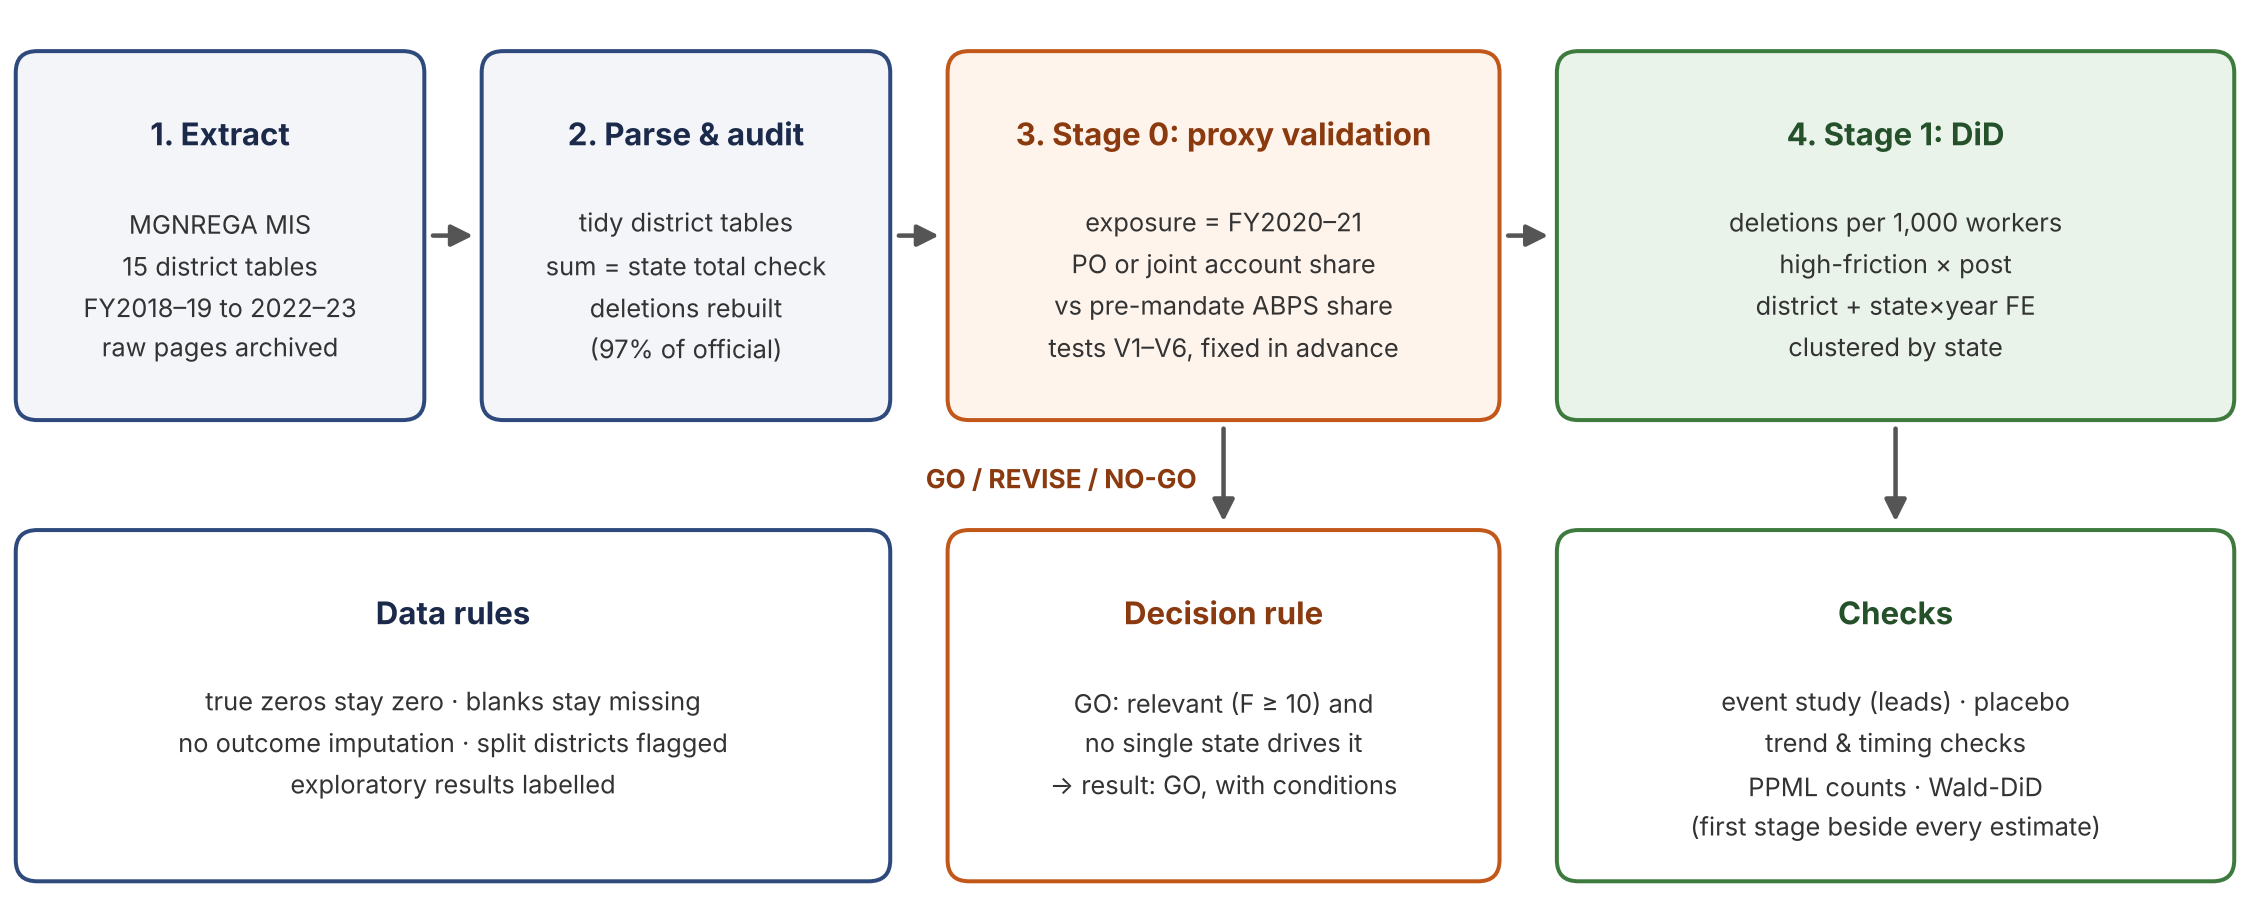
\includegraphics[width=0.92\textwidth]{design.png}
\caption{Overall design: extraction and audit, Stage~0 proxy validation with a pre-set decision rule, Stage~1 difference-in-differences with diagnostics.}\label{fig:design}
\end{figure*}

\subsection{Stage 0: Validating the Exposure Proxy}
For district $d$ in state $s$ we estimate
\begin{equation}
R_{ds} = \pi\, \tilde{E}_{ds} + \alpha_s + u_{ds},
\end{equation}
where $R$ is a readiness measure, $\tilde{E}$ the standardised exposure and $\alpha_s$ state fixed effects; standard errors are clustered by state. Six tests were fixed before any test ran: V1 relevance (correct sign, $p<0.05$, effective $F \ge 10$), V2 components (post-office and joint shares entered together), V3 within-state variation ($\ge$10\% of variance), V4 stability ($r \ge 0.8$ with neighbouring years), V5 balance on pre-period deletions and register size, and V6 leave-one-state-out robustness. The decision rule was GO if V1 and V6 pass, REVISE if the sign is right but the link weak, and NO-GO otherwise. Relevance uses the \emph{pre-mandate} ABPS share of wages, because eligibility snapshots post-date the deletions.

\subsection{Stage 1: Difference-in-Differences}
With $H_d = 1$ for districts in the top within-state decile of exposure and $\text{Post}_t = 1$ from FY2022--23,
\begin{equation}
Y_{dt} = \beta\, (H_d \times \text{Post}_t) + \gamma_d + \delta_{s(d)t} + \varepsilon_{dt},
\end{equation}
where $Y$ is deletions per 1,000 workers, $\gamma_d$ are district and $\delta_{st}$ state-by-year fixed effects, and errors are clustered by state (33 clusters). Following Stage~0 we report exposure quartiles, continuous exposure and its components, a direct readiness gap (1 $-$ FY2021--22 ABPS share), an event study with FY2021--22 as reference, a placebo, a group-specific trend, a check that drops FY2021--22 (timing shift), PPML on deletion counts with log start-of-year stock as offset, and a Wald-DiD $\hat\beta/\hat\pi$ that rescales the effect per 10-point lower ABPS share, with a state-cluster bootstrap (300 draws).

\section{Results}
\subsection{Stage 0: The Proxy Is Relevant but Weak}
Table~\ref{tab:v1} reports V1. In FY2019--20 to FY2021--22, one SD more exposure predicts a 0.13--0.15 SD lower ABPS share of wages, with effective $F$ = 29--65; FY2018--19 falls short ($F$ = 7.8). Dropping each state in turn leaves the coefficient between $-0.11$ and $-0.15$ (all $p<0.001$), so V1 and V6 pass and the rule gives \textbf{GO}. V3 (61\% within-state) and V4 ($r$ = 0.86--0.98) also pass. However, the within-state $R^2$ is only 2.4--3.1\%, the within-state rank version never reaches $F$ = 10, and the binned scatter (Fig.~\ref{fig:bins}) shows that a small group of very high-exposure districts carries the slope. Joint accounts drive the signal in every year (V2). Current eligibility measures show no relationship, as expected for post-treatment data. V5 finds a borderline pre-period gap: high-exposure districts were already deleting slightly more ($+0.16$ SD in FY2020--21, $p=0.07$). We therefore use a high-friction indicator rather than a linear dose.

\begin{table}[t]
\centering\footnotesize
\caption{Stage 0, V1: ABPS share of wages on exposure (SD per SD)}\label{tab:v1}
\begin{tabular}{@{}lrrrrr@{}}
\toprule
Readiness year & Coef. & SE & $F$ & $N$ & $R^2_{w}$\\
\midrule
FY2018--19 & $-0.118$ & 0.042 & 7.8 & 553 & 0.024\\
FY2019--20 & $-0.138$ & 0.026 & 29.0 & 567 & 0.028\\
FY2020--21 & $-0.154$ & 0.019 & 65.3 & 571 & 0.031\\
FY2021--22 & $-0.134$ & 0.017 & 64.3 & 584 & 0.025\\
\bottomrule
\end{tabular}\\[2pt]
{\scriptsize State fixed effects; SEs clustered by state (26--29 states).}
\end{table}

\begin{figure}[t]
\centering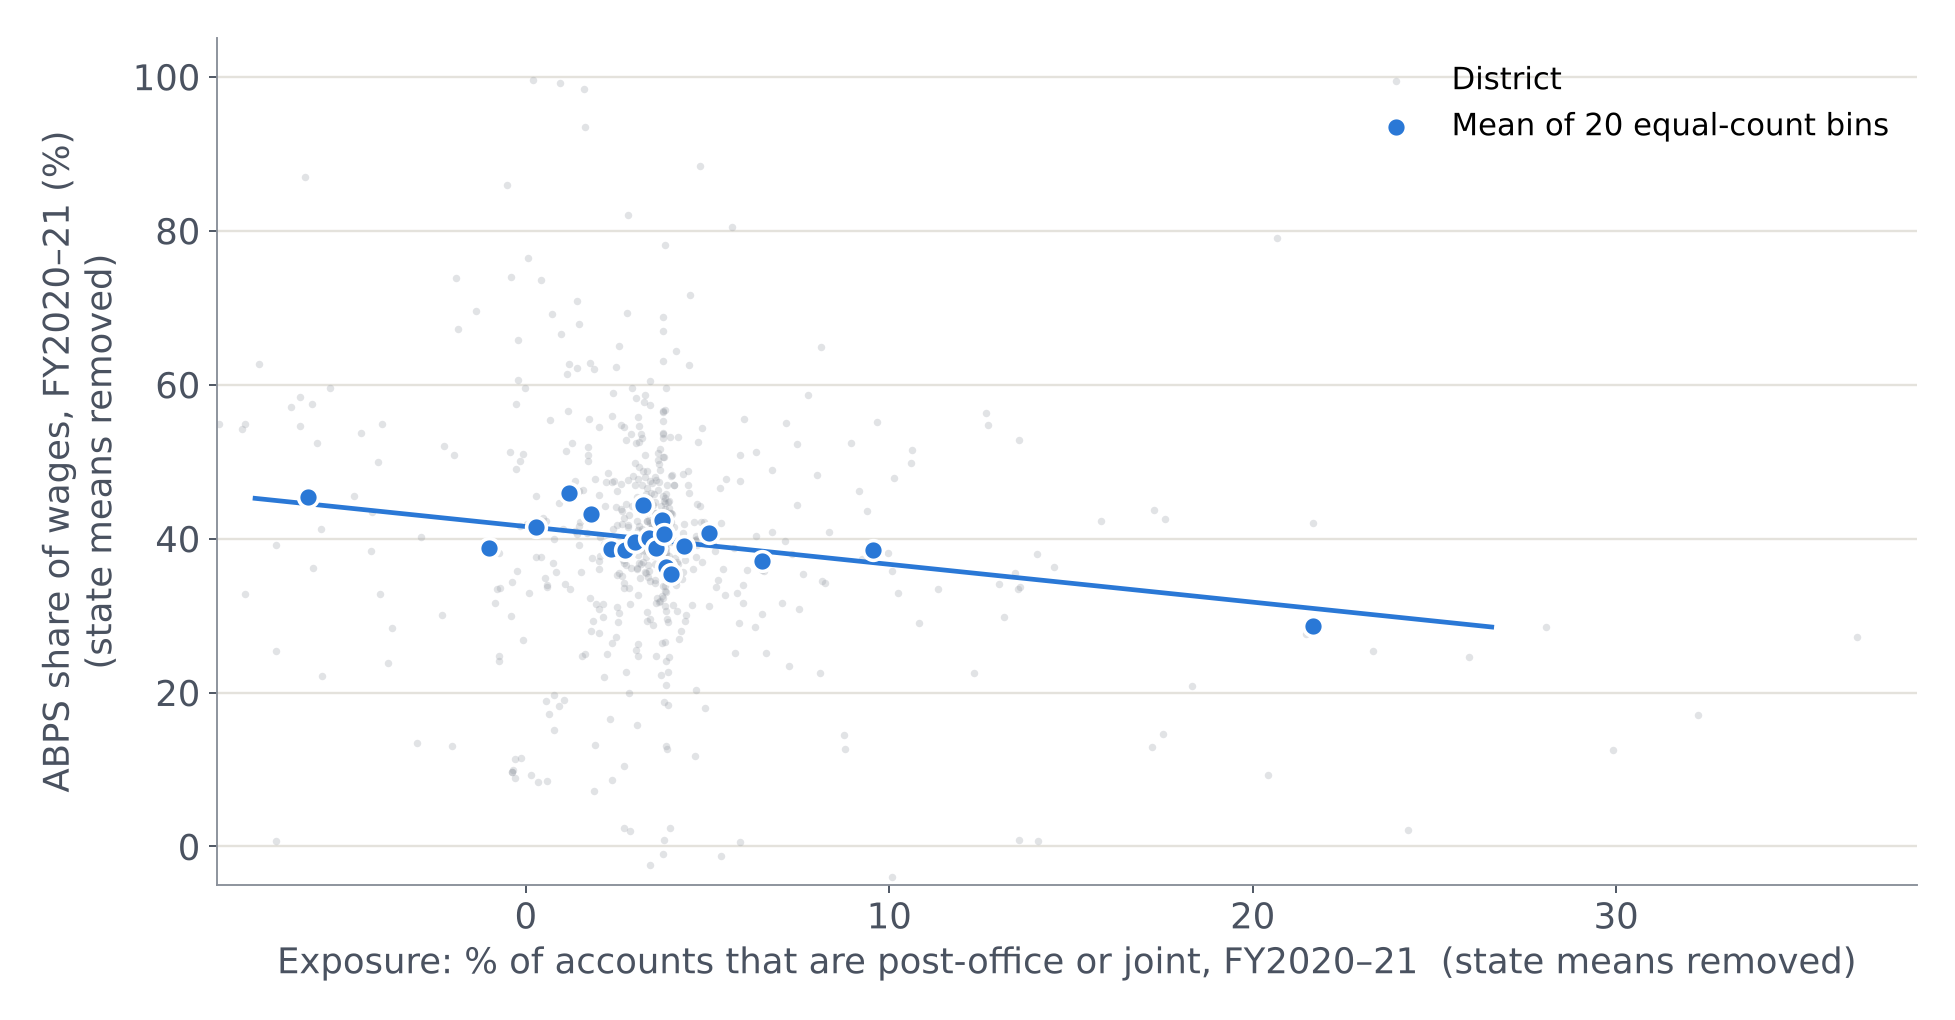
\includegraphics[width=\columnwidth]{binscatter_white.png}
\caption{Stage 0: ABPS share of wages vs exposure, FY2020--21, state means removed (20 equal-count bins).}\label{fig:bins}
\end{figure}

\subsection{Stage 1: No Larger Rise in High-Friction Districts}
Deletions rose from an average of 34 to 120 per 1,000 workers between the pre-period and FY2022--23. High-friction districts already deleted more than the rest of their state before ABPS, but that gap did not widen (Fig.~\ref{fig:trends}). The main estimate is $-1.2$ per 1,000 (SE 9.3, $p = 0.90$, 95\% CI $[-19.4, 17.0]$). Event-study leads are imprecise ($-12.2$ and $+8.7$, largest $|t| = 1.4$), and the FY2022--23 coefficient is $-2.4$ (Fig.~\ref{fig:event}). Table~\ref{tab:did} shows that results are similar across specifications: 12 of 14 are not significant at 5\%. The two exceptions point in opposite directions, with the post-office share alone showing a small rise ($+1.4$ per 1,000 per SD) and the PPML continuous model proportionally fewer deletions ($-14\%$ per SD). High-friction districts had a 6.8-point lower ABPS share before the mandate (first-stage $F$ = 9.3), so the Wald-DiD is $-1.7$ deletions per 1,000 per 10-point lower readiness, with a bootstrap 95\% CI of $[-40.8, 22.1]$: we cannot rule out moderate effects in either direction.

\begin{figure}[t]
\centering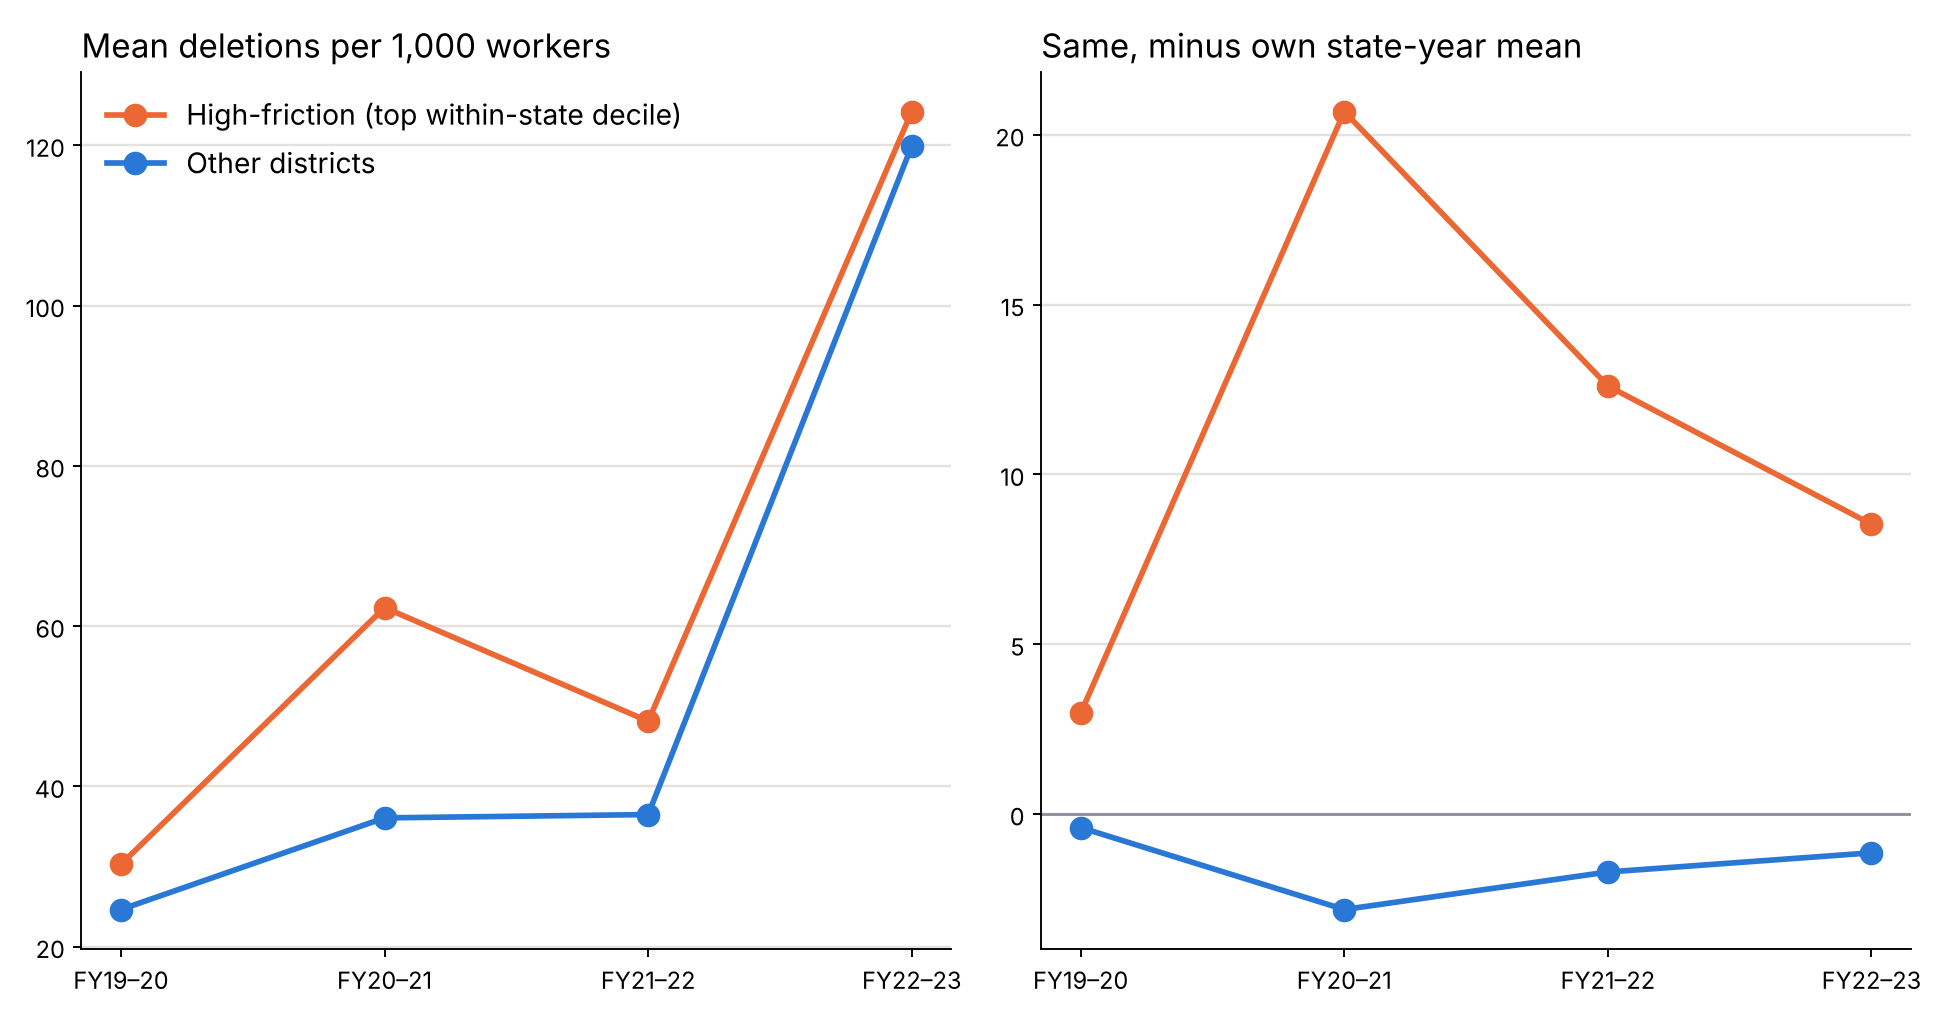
\includegraphics[width=\columnwidth]{fig_raw_trends.png}
\caption{Deletions per 1,000 workers by group: levels (left) and net of state-year means (right).}\label{fig:trends}
\end{figure}

\begin{figure}[t]
\centering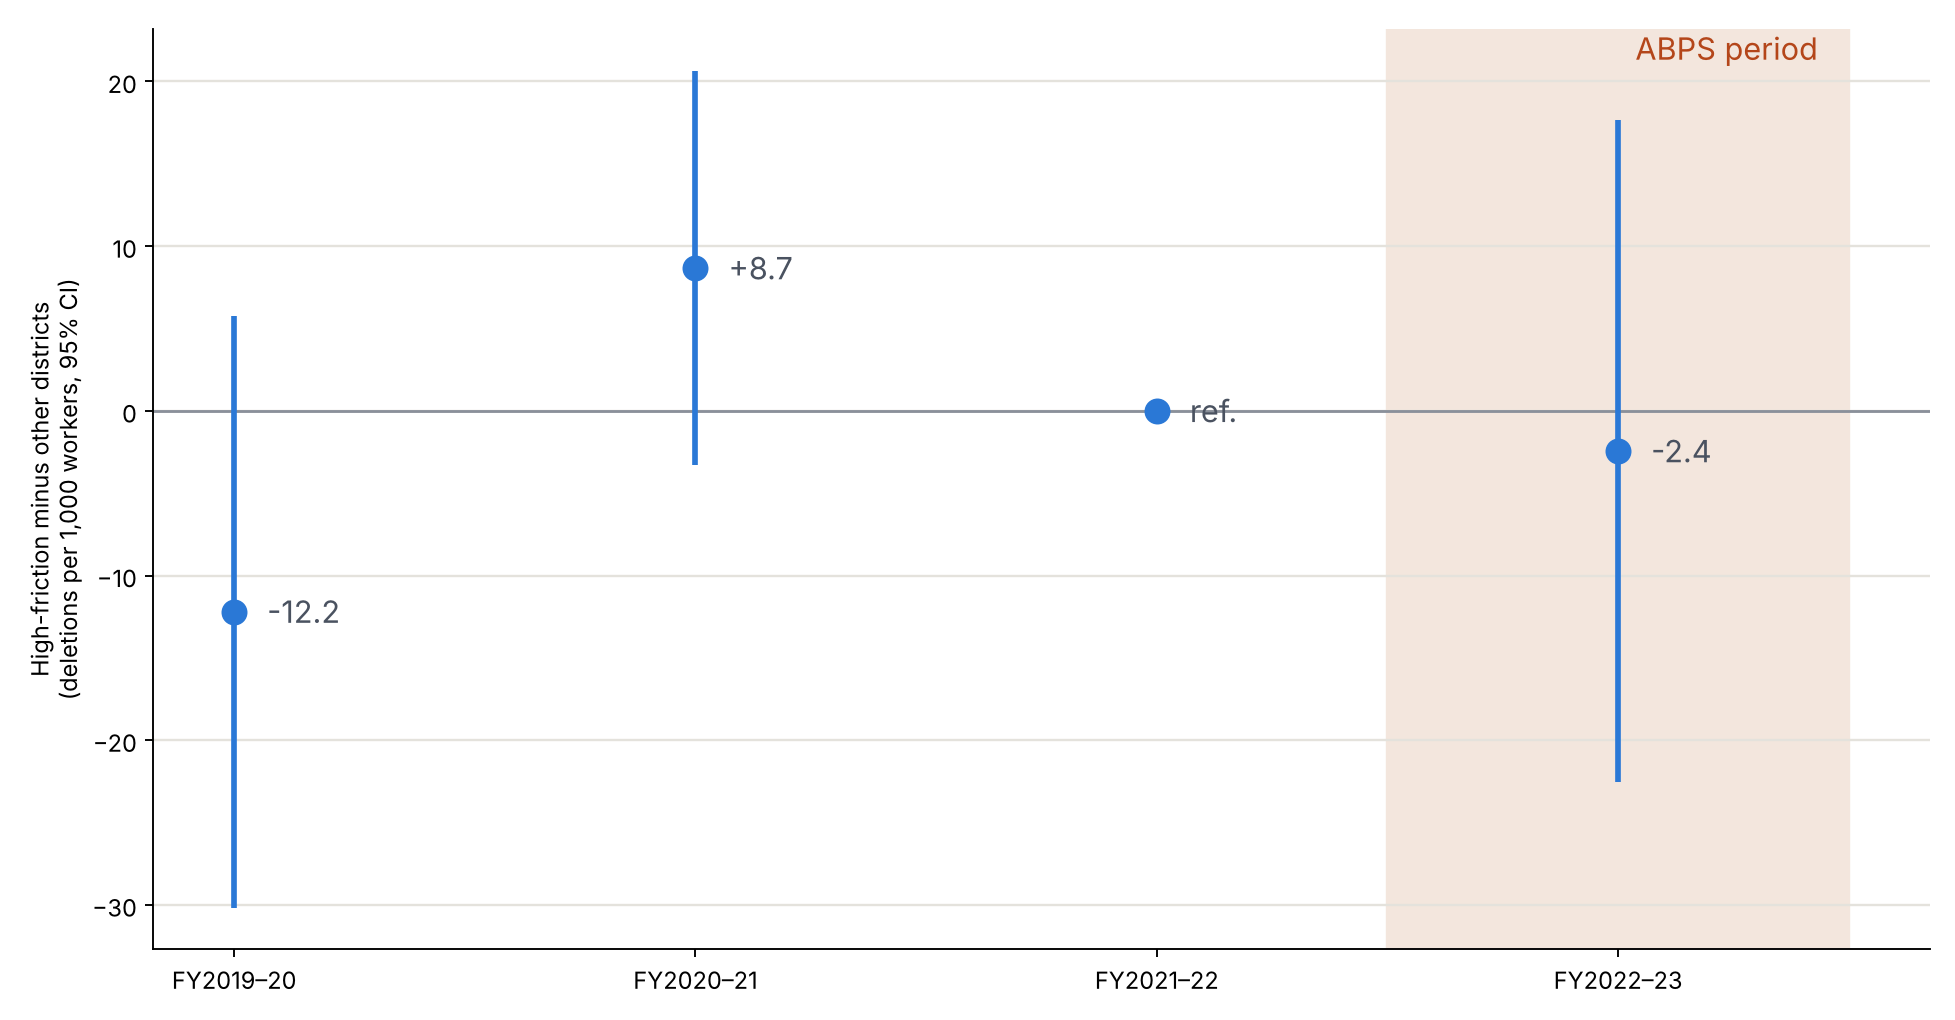
\includegraphics[width=\columnwidth]{fig_event_study.png}
\caption{Event study: high-friction minus other districts, relative to FY2021--22 (95\% CI).}\label{fig:event}
\end{figure}

\begin{table}[t]
\centering\footnotesize
\caption{Stage 1: DiD estimates (deletions per 1,000 workers)}\label{tab:did}
\begin{tabular}{@{}p{4.55cm}rrr@{}}
\toprule
Specification & Coef. & SE & $p$\\
\midrule
High-friction $\times$ post (main) & $-1.18$ & 9.30 & 0.90\\
Quartile 4 vs Q1 $\times$ post & 6.38 & 14.56 & 0.66\\
Continuous exposure (per SD) & $-0.20$ & 2.33 & 0.93\\
Joint-account share (per SD) & $-2.18$ & 3.30 & 0.51\\
Post-office share (per SD) & 1.39 & 0.62 & 0.03\\
Direct readiness gap (per SD) & 3.44 & 8.36 & 0.68\\
Drop FY2021--22 (timing) & $-2.89$ & 9.92 & 0.77\\
With high-friction linear trend & $-13.32$ & 16.07 & 0.41\\
Placebo: FY2021--22 as post & 2.12 & 4.58 & 0.65\\
PPML, high-friction (log points) & $-0.24$ & 0.14 & 0.10\\
PPML, continuous (log points) & $-0.16$ & 0.06 & 0.01\\
Unwinsorised outcome & $-1.95$ & 10.88 & 0.86\\
\bottomrule
\end{tabular}\\[2pt]
{\scriptsize District and state$\times$year FE; SEs clustered by state (33). $N$ = 2,594 (2,185 for the readiness gap).}
\end{table}

\section{Discussion and Limitations}
The proxy passes its pre-set test, but only weakly, and the weak first stage limits what the reduced form can show: a null DiD with a 6.8-point first stage is consistent with no effect and with moderate effects of either sign. Four limits matter most. First, FY2022--23 is the only post-mandate year in our extract; the order arrived in its last two months and became binding in FY2023--24, so the main effect may fall in later years. Second, the MIS and official series disagree on when deletions happened. Third, eligibility exists only as a current snapshot, so it cannot validate the proxy before treatment. Fourth, district splits (for example, Andhra Pradesh from 13 to 26 districts) are dropped rather than mapped. Results are associations under parallel trends and do not establish wrongful exclusion.

\section{Conclusion}
A validated but weak proxy for ABPS conversion friction does not predict a larger rise in MGNREGA worker deletions in FY2022--23. The analysis pipeline, from raw MIS pages to estimates, is reproducible from a single notebook. Next steps are extracting FY2023--24 and FY2024--25, building an LGD-code district crosswalk, adding Census and rainfall covariates, and bounding pre-trends with the method of Rambachan and Roth.

\balance
\begin{thebibliography}{9}\footnotesize
\bibitem{mns2016} K.~Muralidharan, P.~Niehaus, and S.~Sukhtankar, ``Building state capacity: Evidence from biometric smartcards in India,'' \emph{American Economic Review}, vol.~106, no.~10, pp.~2895--2929, 2016.
\bibitem{dcdh2018} C.~de~Chaisemartin and X.~D'Haultf{\oe}uille, ``Fuzzy differences-in-differences,'' \emph{Review of Economic Studies}, vol.~85, no.~2, pp.~999--1028, 2018.
\bibitem{cgs2024} B.~Callaway, A.~Goodman-Bacon, and P.~H.~C. Sant'Anna, ``Difference-in-differences with a continuous treatment,'' NBER Working Paper 32117, 2024.
\bibitem{rr2023} A.~Rambachan and J.~Roth, ``A more credible approach to parallel trends,'' \emph{Review of Economic Studies}, vol.~90, no.~5, pp.~2555--2591, 2023.
\bibitem{bdm2004} M.~Bertrand, E.~Duflo, and S.~Mullainathan, ``How much should we trust differences-in-differences estimates?'' \emph{Quarterly Journal of Economics}, vol.~119, no.~1, pp.~249--275, 2004.
\bibitem{cgz2020} S.~Correia, P.~Guimar\~aes, and T.~Zylkin, ``Fast Poisson estimation with high-dimensional fixed effects,'' \emph{Stata Journal}, vol.~20, no.~1, pp.~95--115, 2020.
\bibitem{mis} Ministry of Rural Development, ``MGNREGA MIS reports,'' \url{https://mnregaweb4.dord.gov.in/netnregarep/MISreport4.aspx}, accessed 29 Oct. 2026.
\bibitem{ls} Lok Sabha, Unstarred Question No.~294, ``Deletion of workers under MGNREGS,'' 4 Feb. 2025.
\end{thebibliography}
\end{document}
